\chapter{Theoretical Background}
\label{sec:theoretical_background}


\section{Molecular Dynamics}

Molecular Dynamics (MD) is a computational method used to simulate the behavior of atoms and molecules over time. In recent years, MD simulations have become essential in many scientific fields, including chemistry, physics, biology, and materials science. Such simulations are used to study various systems, ranging from simple gases and liquids to complex biological molecules and new materials.

MD simulations act on an atomic level and attempt to explain macroscopic properties of a system from the interactions between the individual atoms and molecules. The recent advances in computational power have made it possible to simulate systems with millions of particles over long time scales, allowing researchers to study complex systems in unprecedented detail. Contrary to experimental methods, MD simulations can provide detailed information about the behavior of atoms and molecules, sometimes inaccessible to experimental methods~\cite{Perilla2017}.

Two illustrations of such simulations are shown in \autoref{fig:hiv_capsid} and \autoref{fig:md_simulation_loop}. The first image shows a simulation of the HIV-1 capsid, a protein shell that surrounds the genetic material of the human immunodeficiency virus (HIV). By using a simulation-based approach, researchers were able to study critical properties of the HIV-1 capsid which would be difficult to access using other methods~\cite{Perilla2017}. The second image shows a simulation of shear band formation around a precipitate in metallic glass. This simulation found evidence that depending on the precipitate size, shear bands can either dissolve, wrap around, or be blocked by the precipitate~\cite{Brink2016}. This information is crucial for understanding the mechanical properties of metallic glasses and can be used to design new materials with improved properties.


\begin{multicols*}{2}
      \begin{figure}[H]
            \centering
            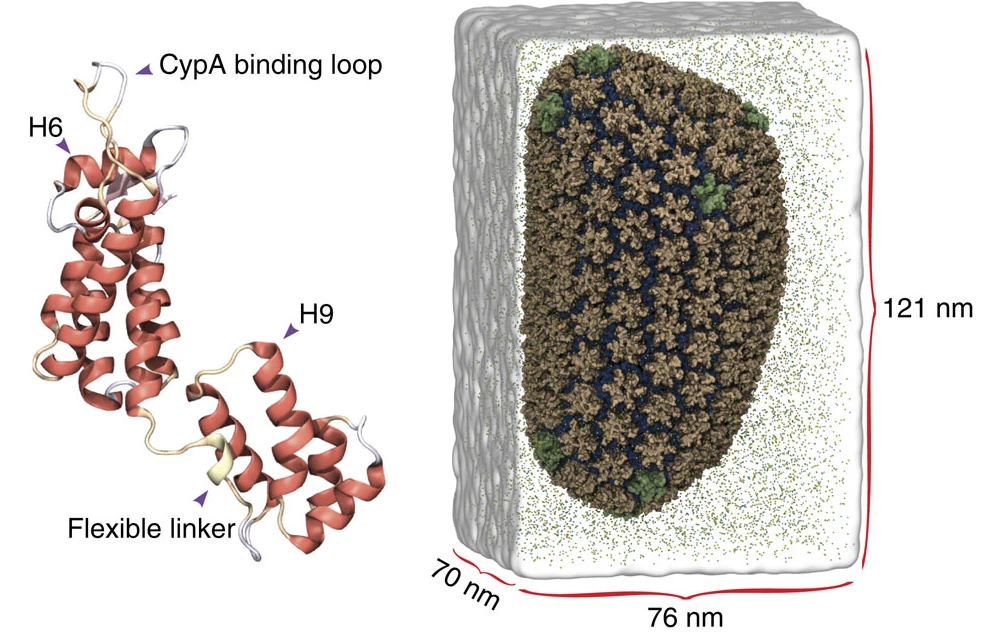
\includegraphics[width=1\columnwidth, trim={0cm 0 0cm 0cm}]{figures/Intro/HIV-1.png}
            \caption{Molecular dynamics simulations of the HIV-1 capsid. Perilla et al.~\cite{Perilla2017} used a simulation containing 64,423,983 atoms to investigate different properties of the HIV-1 capsid at an atomic resolution.}
            \label{fig:hiv_capsid}
      \end{figure}

      \begin{figure}[H]
            \centering
            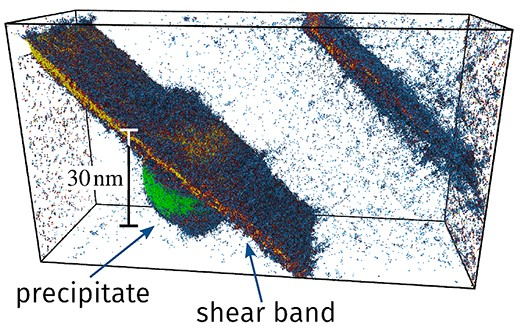
\includegraphics[width=1\columnwidth,trim={0cm 0 0cm 0cm}]{figures/Intro/metallic-glass-crack.jpg}
            \caption{Molecular dynamics simulations of shear band formation around a precipitate in metallic glass, as demonstrated by Brink et al.~\cite{Brink2016}.}
            \label{fig:md_simulation_loop}
      \end{figure}
\end{multicols*}

\subsection{Quantum Mechanial Background}

Our current knowledge of physics suggests that the behavior of atoms and molecules is governed by the laws of quantum mechanics, where particles are described by probabilistic wave functions evolving over time. The physicist Erwin Schrödinger first formulated a mathematical model describing this concept in 1926, which has gotten widespread acceptance and is now known as the Schrödinger equation. The Schrödinger equation is a partial differential equation describing the time evolution of a quantum system. It is given by:

\begin{equation}
      i \hbar \frac{\partial \Psi}{\partial t} = \hat{H} \Psi
\end{equation}

Where $\Psi$ is the system's wave function, $\hat{H}$ is the Hamiltonian operator describing the system's energy, $t$ is the time, and $\hbar$ is the reduced Planck constant.
\smallskip

The Schrödinger equation provides a way to calculate the future states of a quantum system given the current state of the system. However, solving the Schrödinger equation for systems with many particles is computationally very expensive and quickly becomes infeasible for systems with more than a few particles~\cite{Leimkuhler2015}. Simulating a single water molecule consisting of three nuclei and 10 electrons would require solving a partial differential equation with 39 variables (The water molecule consists of two hydrogen atoms, one oxygen atom, and 10 electrons. Each of those 13 objects is described by three spatial coordinates resulting in $(2+1+10)\times 3 = 39$ variables). The can be written as:

\begin{equation}
      i \hbar \frac{\partial \Psi}{\partial t} = -\hbar^2 \sum_{i=1}^{13} \frac{1}{2m_i} \left( \frac{\partial^2 \Psi}{\partial x_i^2} + \frac{\partial^2 \Psi}{\partial y_i^2} + \frac{\partial^2 \Psi}{\partial z_i^2} \right) + U_p (x_1, y_1, z_1, \ldots, x_{13}, y_{13}, z_{13}) \Psi
\end{equation}

In this equation $m_i$ is the mass of the $i$-th object, $x_i$, $y_i$, and $z_i$ are the spatial coordinates of the $i$-th object, and $U_p$ is the potential energy function of the system.
\smallskip

As the Schrödinger equation is a partial differential equation, it is computationally expensive to solve for systems with many particles, as one quickly runs into the curse of dimensionality. The Born-Oppenheimer approximation simplifies this problem by exploiting the significant mass difference between electrons and nuclei. From the perspective of fast-moving electrons, the much heavier nuclei appear nearly stationary, which allows the separation of electronic and nuclear motions and results in treating the nuclei as classical particles. The remaining electronic energies can then be combined further using a new energy function $U$ that depends solely on nuclear positions.
This potential energy surface $U$ is typically obtained through quantum mechanical calculations or fitted to empirical data and is the key component of molecular dynamics simulations.

As the Born-Oppenheimer approximation is based on simplifications of the full model, it is not always accurate. Depending on the system under investigation and the chosen potential energy function $U$, it is possible that the Born-Oppenheimer approximation neglects certain quantum mechanical effects, resulting in inaccuracies in the simulation.

Despite these limitations, the Born-Oppenheimer approximation is widely used in molecular dynamics simulations and is the best-known method to simulate systems with many particles.

\subsection{Classical Molecular Dynamics}

After applying the Born-Oppenheimer approximation and using Newton's second law of motion, the Schrödinger equation can be transformed into a system of ordinary differential equations of the form:

\begin{align}
      m_i \frac{d^2 x_i}{dt^2} & = -\frac{\partial U}{\partial x_i} \\
      m_i \frac{d^2 y_i}{dt^2} & = -\frac{\partial U}{\partial y_i} \\
      m_i \frac{d^2 z_i}{dt^2} & = -\frac{\partial U}{\partial z_i}
\end{align}

Where $m_i$ is the mass of the $i$-th particle, $x_i$, $y_i$, and $z_i$ are the spatial coordinates of the $i$-th particle, and $U$ is the potential energy function of the system. Using vector notation, this system of equations can be written as:

\begin{equation}
      m_i \frac{d^2 \vec{r}_i}{dt^2} = -\nabla_i U
\end{equation}

These equations look exactly like Newton's second law of motion, where the force acting on the $i$-th particle is given by the gradient of the potential energy function $U$. This allows us to simulate the behavior of the system by solving the equations of motion for each particle over time.

\subsection{Numerical Integration}

Since the simulation domain potentially consists of a vast number of particles all interacting with each other, it is generally not possible to solve the equations of motion analytically. This problem is known under the N-body problem, and it can be shown that there are no general solutions for systems with more than two particles. It is, however possible to approximate solutions of these equations of motion using numerical integration methods. A standard method for solving such systems is the Verlet algorithm. This integration scheme is derived from the Taylor expansion of the position of the $i$-th object $\vec{r}_i$ at time $t - \Delta t$ and $t + \Delta t$ and is given by:

\begin{equation}
      \vec{r}_i(t + \Delta t) = 2 \vec{r}_i(t) - \vec{r}_i(t - \Delta t) + \vec{a}_i(t) \Delta t^2
\end{equation}

Where $\vec{a}_i(t)$ is the acceleration of the $i$-th object at time $t$. This acceleration can be calculated from the particle mass and the acting forces using Newton's second law of motion $\vec{a}_i(t) =\frac{F_i}{m_i}= \frac{-\nabla_i U}{m_i}$.

\subsection{Potential Energy Function}

As stated above, the potential energy function $U$ is a critical component of molecular dynamics simulations as it fundamentally defines the properties of the system. MD simulations use many different potential energy functions, all of which are tailored to describe specific aspects of the system. Those potentials typically use a mixture of 2-body, 3-body, and 4-body interactions between the particles each used to describe different aspects of particle interactions. The 2-body interactions typcially express the effect of Pauli repulsion, atomic bonds, and coulomb interactions, while higher-order interactions allow for asymmetric wave functions for atoms in bound groups \cite{Leimkuhler2015}.

A common choice for the potential energy function is the Lennard-Jones potential. The simplicity of the Lennard-Jones potential makes it a popular choice for many systems, as it can be computed quite efficiently, while still capturing many of the essential properties of the system. The Lennard-Jones potential is given by:

\begin{equation}
      U_{LJ}(r) = 4 \epsilon \left[ \left( \frac{\sigma}{r} \right)^{12} - \left( \frac{\sigma}{r} \right)^6 \right]
\end{equation}


Where $r$ is the distance between the particles, $\epsilon$ is the depth of the potential well, and $\sigma$ is the distance at which the potential is zero. The parameters $\epsilon$ and $\sigma$ can differ for each type of particle interaction and are either determined from theoretical considerations of the material or fitted to experimental data.

\subsection{Simulation Loop}

Using the methods described above, it is possible to simulate the behavior of a system of particles over time. The general simulation loop for a molecular dynamics simulation can be described as follows:

\begin{enumerate}
      \item \textbf{Initialization} \\
            The simulation starts by initializing the positions and velocities of the particles. The initial positions and velocities can be chosen randomly or based on experimental data, depending on the system under investigation.

      \item \textbf{Position Updates} \\
            In this step, the positions of the particles are updated using a numerical integration scheme such as the Verlet algorithm.

      \item \textbf{Force Calculation} \\
            The forces acting on the particles are calculated based on the current positions of the particles and the chosen potential energy function $U$.

      \item \textbf{Acceleration and Velocity Updates} \\
            The acceleration of each particle is calculated using Newton's second law of motion and the forces acting on the particles. The velocities of the particles are then updated accordingly.

      \item \textbf{External Forces and Constraints} \\
            In this step, the simulation can be modified by applying external forces or constraints to the particles. For example, it is possible to introduce boundary conditions, temperature control, or other outside influences to the simulation.

      \item \textbf{Update Time and Repeat} \\
            The simulation time is updated, and the simulation loop (steps 2-5)
            are repeated until the desired simulation time is reached. The collected data can then be analyzed to study properties of the system.
\end{enumerate}


Many different software packages exist to perform such simulations. Some widely used examples of such systems are LAAMPS\footnote{\url{https://lammps.sandia.gov/}} and GROMACS\footnote{\url{https://www.gromacs.org/}}. Both attempt to efficiently solve the underlying N-body problem and provide the user with a high-level interface to specify parameters and properties of the simulation.

Many different approaches exist to efficiently solve the N-body problem, and no single best approach works well for all systems as the optimal implementation heavily depends on the simulation state the hardware used to perform the simulation. However, LAAMPS and GROMACS use a single implementation and therefore cannot adapt their algorithms to the current simulation state.

In the following section, we will introduce AutoPas, a library designed to efficiently deal with evolving particle simulations, built on the concept of automatically switching between different implementations to achieve the best performance for the current simulation state.

\section{AutoPas}

AutoPas is an open-source library designed to achieve optimal node level performance for short-range particle simulations. On a high level, AutoPas can be seen as a black box performing arbitrary N-body simulations with short-range particle interactions. However, AutoPas differentiates itself from other libraries by providing many different algorithmic implementations for the N-body problem, each with different performance and memory usage trade-offs. No single implementation is optimal for all simulation scenarios and can change over time~\autoref{GRATL2022108262}, consequently, AutoPas is designed to be adaptive and can periodically switch between different implementations to remain reasonably close to the current optimal configuration.

Since AutoPas just provides a high-level interface for short-range N-body simulations. It is left to the user to specify the desired model and parameters of the simulation. Fortunately, AutoPas also provides some example implementations, such as \texttt{\gls{mdflexible}}. \texttt{\gls{mdflexible}} is a simple molecular dynamics framework built on top of AutoPas that allows users to specify the desired simulation parameters and run simulations. In this work we will primarily focus on \texttt{\gls{mdflexible}} but the concepts can be easily transferred to other simulation frameworks.

\subsection{Autotuning in AutoPas}

AutoPas internally alternates between two phases of operation. The first phase is the \emph{tuning phase}, where AutoPas tries to find the best configuration of parameters which minimize a chosen performance metric (e.g., time, energy usage) for the current simulation state. This is achieved by trying out different configurations of parameters and measuring their performance. The configuration that optimizes the chosen performance metric is then used in the following \emph{simulation phase},assuming that the optimal configuration found in the tuning phase still performs reasonably well during this phase.
As the simulation progresses and the characteristics of the system change, the previously chosen configuration can drift arbitrarily far from the actual optimal configuration. To counteract this, AutoPas periodically alternates between tuning and simulation phases to ensure that the used configuration remains close to the optimal configuration.

The power of AutoPas comes from its vast amount of tunable parameters and the huge search space associated with them. Other software packages such as LAAMPS and GROMACS are limited to just one implementation and can therefore operate outside of the theoreticaly achievable performance regime.

In the following section, we will discuss the tunable parameters in AutoPas and the different tuning strategies available to find the best configuration of parameters for the current simulation state.

\subsection{Tunable Parameters}

AutoPas currently provides six tunable parameters, which can mostly\footnote{There are some exceptions as some choices of parameters are incompatible with each other.} be combined freely with eachoter. A collection of parameters is called a \emph{Configuration}, and the set of all possible configurations is called the \emph{Search Space}. Each configuration consists of the following parameters:

\begin{enumerate}[label=\textbf{\arabic*.}]
      \item \textbf{Container Options:} \\
            The container options are related to the data structure used to store the particles. The most important categories of data structures in this section are:
            \begin{enumerate}
                  \item \textbf{DirectSum} \\
                        DirectSum does not use any additional data structures to store the particles. Instead, it simply holds a list of all particles. Consequently it needs to rely on brute-force calculations of the forces between all pairs of particles. This results in a complexity of $O(N^2)$ distance checks in each iteration. This inferior complexity renders it completly useless for larger simulations.\\
                        \textit{Generally should not be used except for tiny systems or demonstration purposes.~\cite{VICCIONE2008625}}
                  \item \textbf{LinkedCells} \\
                        LinkedCells segments the domain into a regular cell grid and only considers interactions between particles from neighboring cells. This results in the trade-off that particles further away are not considered for the force calculation. In practice this is not a big issue, as all short-range forces drop off very quickly with distance anyway.
                        LinkedCells also provides a high cache hit rate as particles inside the same cell can be stored contiguously in memory. Typically, the cell size is chosen to be equal to the force cutoff radius $r_c$, meaning that each particle only needs to check interactions between particles inside the $3\times3\times3$ cell grid around the current cell. All other particles are guaranteed to be further away than the cutoff radius and therefore cannot contribute to the acting forces.
                        This reduction in possible interactions can result in a complexity of just $O(N)$ distance checks in each iteration if the particles are spread evenly. There is however still room for improvement as the constant overhead factor can be pretty high, as most distance checks performed by LinkedCells still do not contribute to the force calculation. Due to the uneven scaling of sphere and cube volumes, only about 15.5\% of all particles present in the $3\times3\times3$ cell grid around a particle are within the cutoff radius ~\cite{GRATL2019748}.\\
                        \textit{However, still generally good for large, homogeneous\footnote{Homogeneous in this context, the particles are distributed evenly across the domain.} systems.}

                  \item \textbf{VerletLists} \\
                        VerletLists are another approach to creating neighbor lists for the particles. Contrary to LinkedCells, VerletLists does not rely on a regular grid but instead uses a spherical region around each particle to determine its relevant neighbors. The algorithm creates and maintains a list of all particles present in a sphere within radius $r_c \cdot s$ around each particle, where $r_c$ is the cutoff radius and $s>1$ is the skin factor allowing for a buffer zone around the cutoff radius.
                        By choosing a suitable buffer zone, such that no fast-moving particle can enter the cutoff radius unnoticed, it is possible to only recalculate the neighbor list every few iterations. This method also results in a complexity of $O(N)$ distance checks in each iteration, but provides a way higher interaction rate between particles of $1/s^3$. Ideally, the skin factor should be chosen such the ratio is close to 1, resulting in basically no unnecessary distance checks. This however reduces the buffer zone around the cutoff radius, meaning that the neighbor list needs to be updated more frequently, or the simulation needs to be run at higher temporal precision to remain accurate. Finding a good balance between the two is therefore of great importance.\\
                        \textit{Generally good for large systems with high particle density.}

                  \item \textbf{VerletClusterLists} \\
                        VerletClusterLists differ from regular VerletLists in the way the neighbor lists are stored. Instead of storing the neighbor list for each particle separately, $n_{cluster}$ particles are grouped into a so-called \emph{cluster}, and a single neighbor list is created for each cluster. This reduces memory overhead as the neighbor list only needs to be stored once for each cluster. Whenever two clusters are close, all interactions between the particles in the two clusters are calculated. This also results in a complexity of $O(N)$ distance checks in each iteration but provides the advantage of greatly reduced memory usage compared to regular VerletLists.\\
                        \textit{Generally suitable for large systems with high particle density}

            \end{enumerate}

            \begin{figure}[H]
                  \centering
                  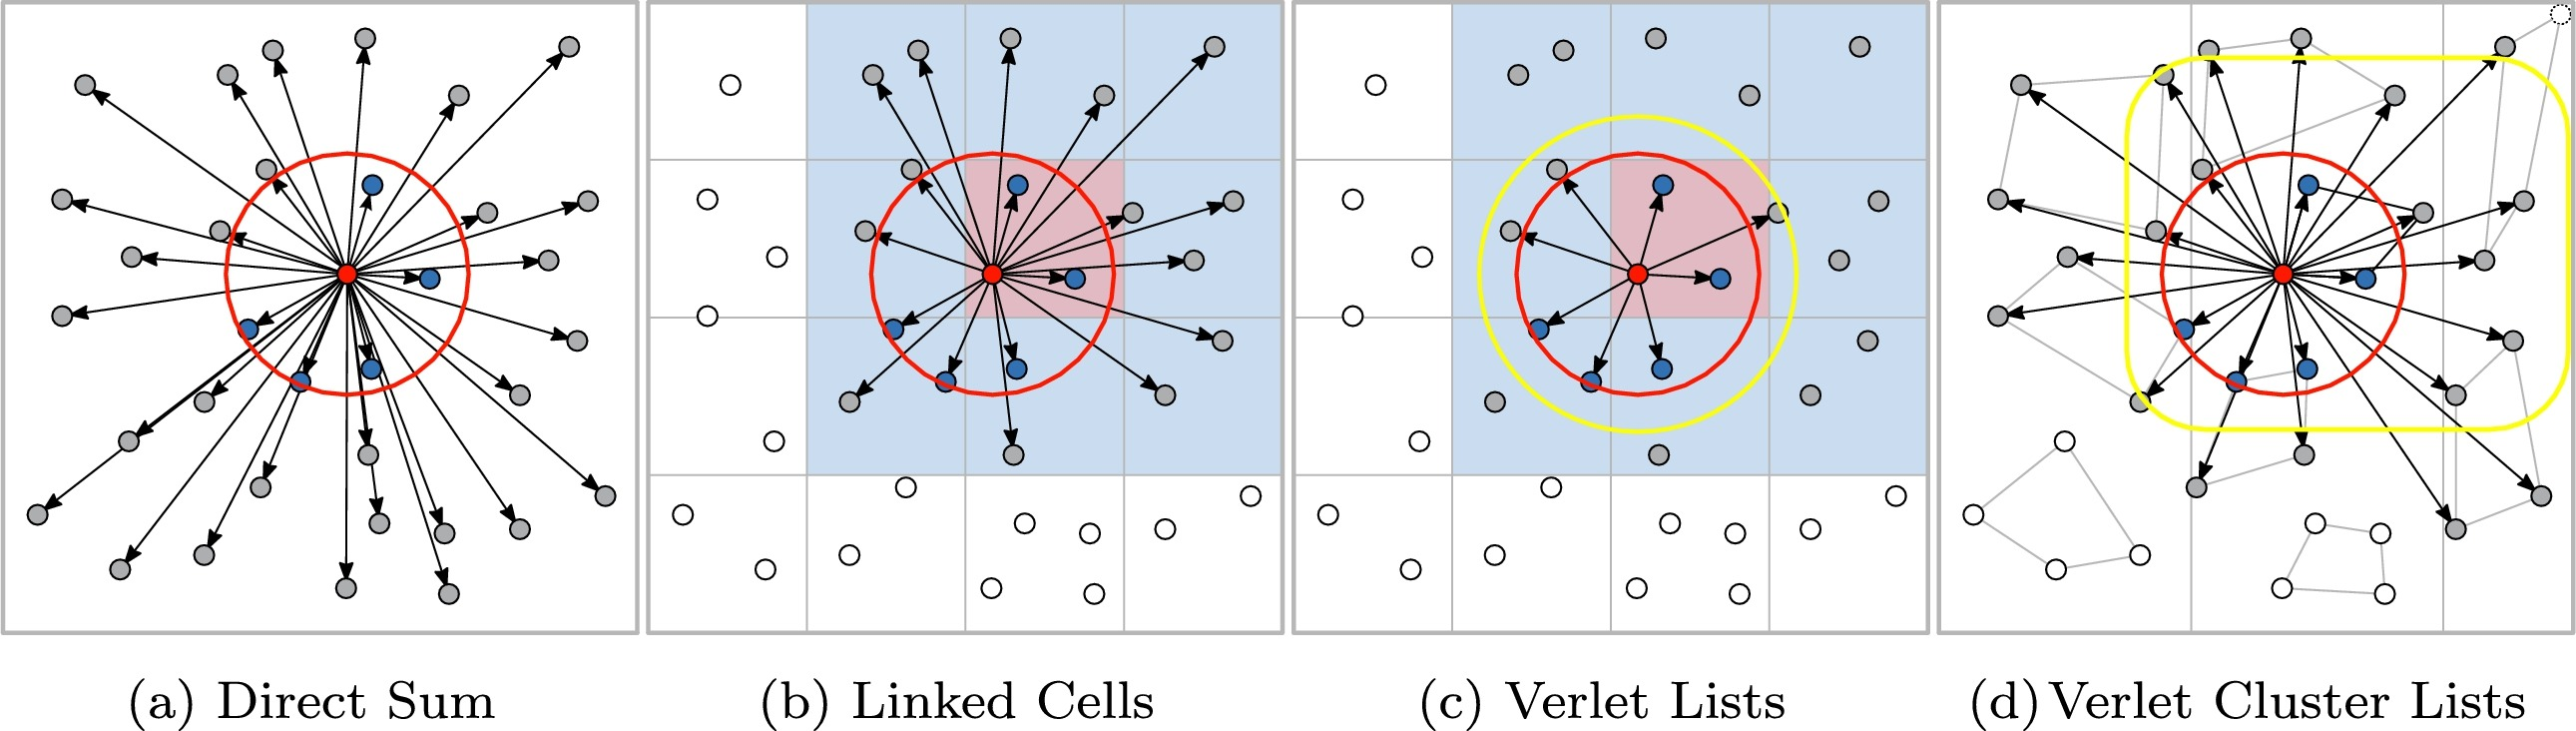
\includegraphics[width=0.8\columnwidth]{figures/Intro/containers.jpg}
                  \caption{Visualization of different container options. \small{Source: Gratl et al.~\cite{GRATL2022108262}}}
                  \label{fig:containers}
            \end{figure}

      \item \textbf{Load Estimator Options:} \\
            The Load Estimator Options are related to the way the simulation behaves in a parallelized setting. The load estimator is responsible for estimating the computational load of each MPI rank and guides the load balancing of the simulation. In this thesis, however, we will not further describe the Load Estimator Options as we primarily focus on the tuning aspect of single-node simulations.

      \item \textbf{Traversal Options:} \\
            These options are related to the traversal algorithm used to calculate the forces between the particles. The traversal determines the order in which the particles are visited and how the forces are applied to the particles. Furthermore, traversal options should prevent race conditions when using multiple threads and can automatically provide load balancing at the node level~\cite{SECKLER2021101296}.

            Some avaialble traversal options are:

            \begin{enumerate}

                  \item \textbf{Sliced Traversal} \\
                        Sliced Traversal is a way to parallelize the force calculation by dividing the domain into different slices and assigning each slice to a different thread. When the slices are chosen correctly, no two threads can work on cells with common neighbors, allowing for the force calculation to be parallelized easiliy, even when using Newtons third law. However on boundaries, the threads need to be synchronized using locks~\cite{GRATL2022108262} to prevent data races.

                  \item \textbf{Colored Traversal} \\
                        Since both LinkedCells and VerletLists only consider interactions with particles from neighboring cells/particles, it is possible to parallelize the force calculation by calculating forces for particles in different cells in parallel. When using Newtons third law however, this is only possible if all simultaneously calculated particles do not share common neighbors, as updating common neighbors could introduce data races when multiple threads act at the same time. This is where the concept of coloring comes into play. Coloring is a way to assign a color to each cell in such a way that cells with the same color do not share common neighbors. This allows for the force calculation of particles in cells with the same color to be parallelized trivially, as data races are impossible. Some ways to color the domain are:
                        \begin{itemize}
                              \item \textbf{C01} \\
                                    The C01 traversal doesn't use any coloring at all, and simply divides the cells to availabe threads. This method is embarrassingly parallel, but comes at the cost of being incompatible with the Newton 3 optimization, as there is no way of preventing data races. As a result, the forces between all pairs of particles are calculated twice, once for each particle. Resulting in a constant overhead of factor 2.

                              \item \textbf{C18} \\
                                    The C18 traversal is a more sophisticated way of coloring the domain. The domain is divided into 18 colors, so no two neighboring cells share the same color. This method also utilizes the Newton 3 law to reduce the number of force calculations. This is achieved by only computing the forces with forward neighbors (neighbors with greater index.) ~\cite{GRATL2022108262}

                              \item \textbf{C08} \\
                                    The C08 traversal is closely related to the C18 traversal, but only uses 8 colors. Due to the fewer colors, there is less synchronization overhead, and a higher degree of parallelism can be achieved. Newton 3 can be used to reduce the number of force calculations
                        \end{itemize}

                        \begin{figure}[H]
                              \centering
                              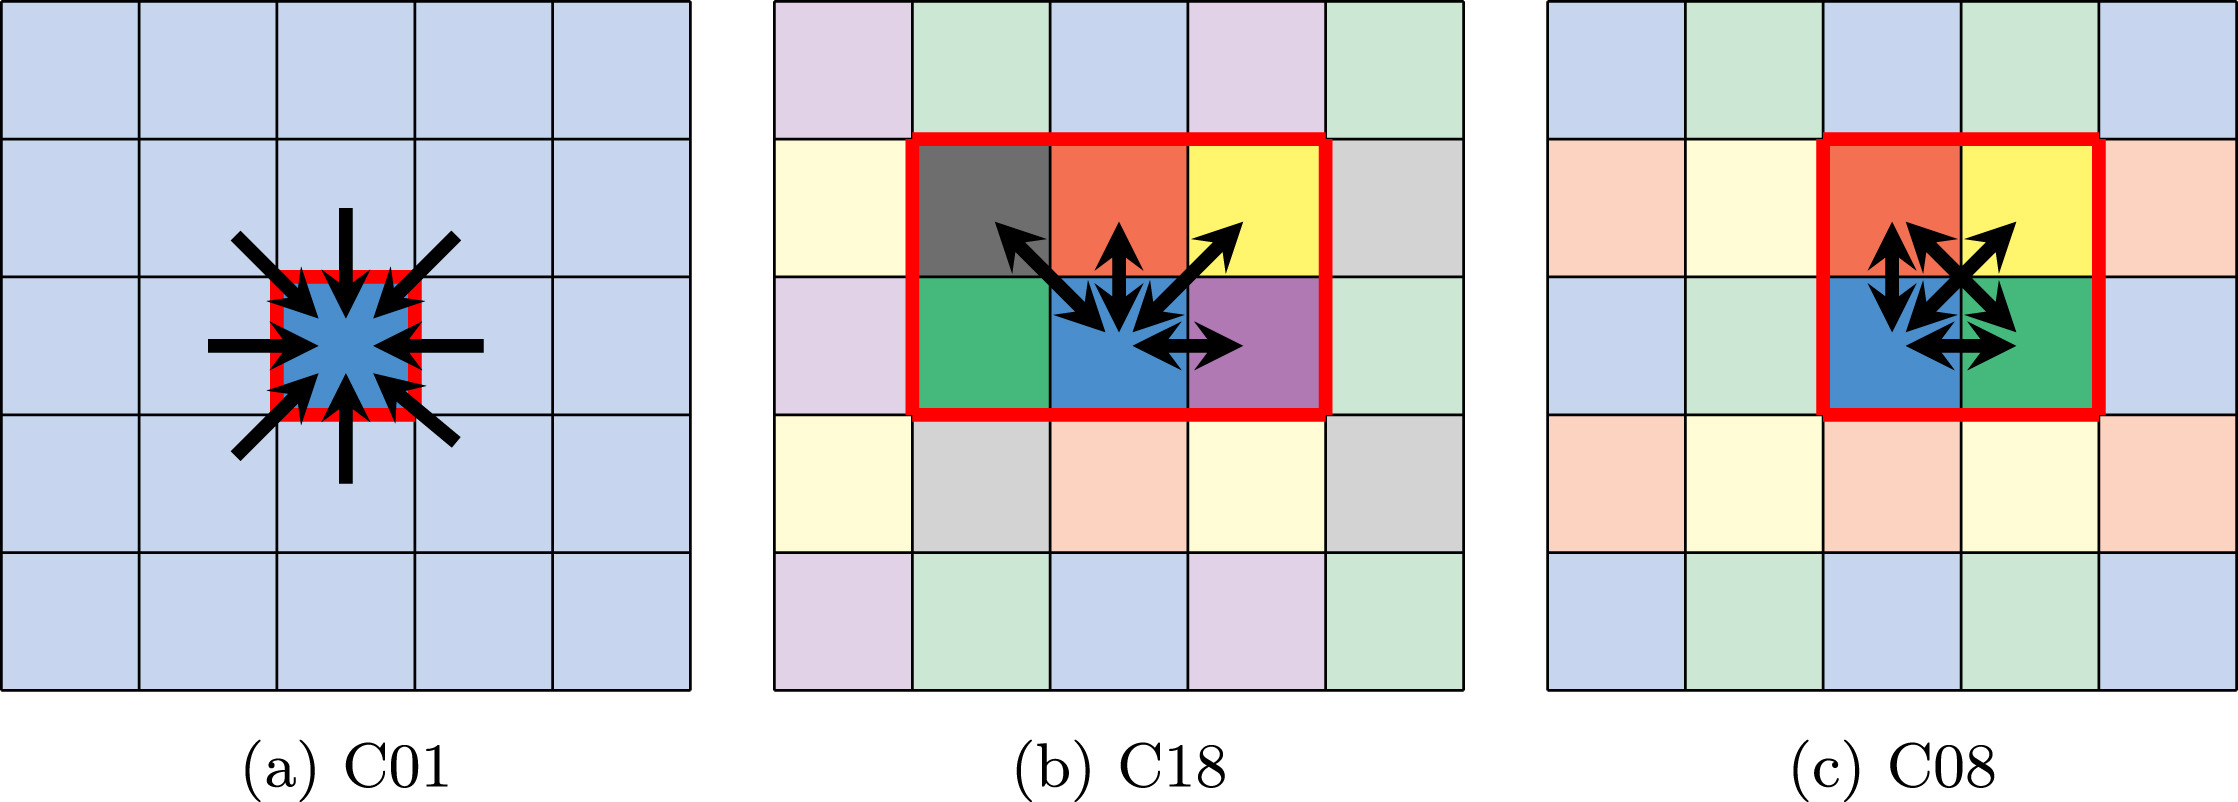
\includegraphics[width=0.7\columnwidth]{figures/Intro/traversals.jpg}
                              \caption{Visualization of different color based traversal options. \small{Source: Newcome et al.~\cite{Newcome2023}}}
                              \label{fig:traversals}
                        \end{figure}

            \end{enumerate}


      \item \textbf{Data Layout Options:} \\
            The Data Layout Options determine how the particles are stored in memory. The two possible data layouts are:
            \begin{enumerate}
                  \item \textbf{SoA} \\
                        The SoA (Structure of Arrays) data layout stores the particles' properties in separate arrays. For example, all particles' x-,y- and z-coordinates are stored in separate arrays. This data layout is beneficial for vectorization as the properties of the particles are stored contiguously in memory. This allows for efficient vectorization of the force calculations as the properties of the particles can be loaded into vector registers in a single instruction.

                  \item \textbf{AoS} \\
                        The AoS (Array of Structures) data layout stores all particle properties in different structures. This allows for efficient cache utilization when working on particles as all properties are close to each other in memory. However, this data layout is not beneficial for vectorization as the same properties of different particles are not stored contiguously in memory. Consequently they need to be loaded into vector registers one by one, which can result in inefficient vectorization of the force calculations.
            \end{enumerate}

      \item \textbf{Newton 3 Options:} \\
            The Newton 3 Options relate to how the forces between the particles are calculated. Newtons third law states that for every action, there is an equal and opposite reaction. Meaning that the magnitude of force between two particles is the same, regardless of which particle is the source and which is the target. In Molecular Dynamics simulations, this rule can be exploited to reduce the number of force calculations by a factor of 2. The two possible Newton 3 options are:
            \begin{enumerate}
                  \item \textbf{Newton3 Off} \\
                        If Newton 3 is turned off, the forces between all pairs of particles are calculated twice, once for each particle. This results in a constant overhead of factor 2.

                  \item \textbf{Newton3 On} \\
                        If Newton 3 is turned on, the forces between all pairs of particles are calculated only once. There is no more overhead due to recalculating the forces twice, but turning on Newton 3 requires additional bookkeeping, especially in multi-threaded environments. This results in more complicated traversal algorithms and can result in a performance overhead.\\
                        \textit{Generally should be turned on whenever available.}
            \end{enumerate}

      \item \textbf{Cell Size Factor:} \\
            The Cell Size Factor is a parameter that is used to determine the size of the cells in the LinkedCells-Container\footnote{The option is also relevant for other containers such as VerletLists as those configurations internally also build their neighbor lists using a Cell Grid}. The cell size factor is typically chosen to be equal to the cutoff radius $r_c$, meaning that each particle only needs to check the forces with particles inside the $3\times3\times3$ cell grid around it as all other particles are guaranteed to be further away than the cutoff radius. We saw in the previous section that this could result in a high number of unnecessary distance checks. By choosing smaller cell sizes, the number of unnecessary distance checks can be reduced. However, the increased overhead of managing more cells can quickly offset the performance gain. And a trade-off between the two needs to be found.

\end{enumerate}

\subsection{Tuning Strategies}

Tuning strategies are the heart of AutoPas and attempt to efficiently find the best parameters for the current simulation state.

The default tuning strategy in AutoPas uses a brute-force approach to find the best parameters for the current simulation state by trying out all possible combinations of parameters and choosing the one performes best. This approach is called \emph{Full Search} and is guaranteed to find the best parameters for the current simulation state. However, it is typically very costly in terms of time and resources as it has to spend a lot of time measuring bad parameter combinations. This is a big issue as the number of possible parameter combinations grows exponentially with the number of parameters and many of them potentially perform very poorly. This makes the full search approach infeasible, especially if more tunable options are added to AutoPas.

To overcome this issue, AutoPas provides a couple of different tuning strategies that can be used to reduce the number of parameter combinations that need to be tested. This is generally achieved by allowing the tuning strategy to modify the queue of parameters that need to be tested, allowing them to exclude unlikely configurations from the testing process.

Develop tuning strategies that can effectively prune the search space is of utmost importance, as bad parameter choices can result in a significant slowdown of the simulation. In the following section, we will introduce the currently available tuning strategies in AutoPas.

\begin{enumerate}
      \item \textbf{Full Search} \\
            The Full Search strategy is the default tuning strategy in AutoPas. It tries out all possible combinations of parameters and chooses the one that optimizes the chosen performance metric. It is guaranteed to find the best parameters for the current simulation state, but as mentioned before, it is very costly.

      \item \textbf{Random Search} \\
            The Random Search strategy is a simple tuning strategy that randomly samples a given number of configurations from the search space and chooses the one that optimizes the chosen performance metric. This approach is faster than the Full Search strategy as it does not need to test all possible combinations of parameters. However, it does not guarantee to find the best parameters for the current simulation state.

      \item \textbf{Predictive Tuning} \\
            The Predictive Tuning strategy attempts to extrapolate previous measurements to predict how the configuration would perform in the current simulation state. It filters the search space and only keeps configurations predicted to perform reasonably well. The extrapolations are accomplished using methods such as linear regression or constructing polynomial functions through the data points.

      \item \textbf{Bayesian Search} \\
            Two implementations of Bayesian tuning exist in AutoPas. Those methods apply Bayesian optimization techniques to predict suitable configurations using performance evidence from previous measurements.

      \item \textbf{Rule Based Tuning} \\
            The Rule Based Tuning strategy uses a set of predefined rules to automatically filter out configurations that are expected to perform poorly. The rules are built on expert knowledge and could look like this:
            \begin{small}
                  \begin{verbatim}
            if numParticles < lowNumParticlesThreshold:
                  [dataLayout="AoS"] >= [dataLayout="SoA"] with same 
                        container, newton3, traversal, loadEstimator;
            endif
            \end{verbatim}
            \end{small}
            The rule states that the data layout "AoS" is generally better than "SoA" if the number of particles is below a certain threshold. The rule-based method can be very effective if the rules are well designed.
\end{enumerate}


This thesis aims to extend these tuning strategies with a new approach based on Fuzzy Logic. Conceptually, this new fuzzy logic-based tuning strategy is very similar to the rule-based tuning strategy as it uses expert knowledge of fuzzy rules to prune the search space. However, contrary to classical rules, fuzzy logic can deal with imprecise and uncertain information, which allows it to only partially activate rules depending on the truthiness value of the condition.
All the suggestions can then be combined based on their degree of activation rather than just following the binary true/false logic. This allows for a more nuanced approach and allows the tuning strategy to interpolate the effect of many different rules to choose the best possible configuration, even if there is no direct rule for this specific case.

In the following section, we will introduce the basic concepts of fuzzy logic.


\section{Fuzzy Logic}

Fuzzy Logic is a mathematical framework that allows for reasoning under uncertainty. It is an extension of classical logic and extends the concept of binary truth values ($true$ and $false$) to a continuous range of truth values in the interval $[0, 1]$. This allows for a more nuanced representation of the truth values of statements, which can be beneficial when dealing with imprecise or uncertain information. Instead of just having true or false statements, it is now possible for statements to be, for example, 40\% true. This concept is beneficial when modeling human language, as the words tend to be imprecise. For example, \emph{hot} can mean different things to different people. For some people, a temperature of 30 degrees Celsius might be considered \emph{hot}, while for others, a temperature of 40 degrees Celsius might be considered \emph{hot}. There is no clear boundary between what is considered hot and what is not, but rather a gradual transition between the two. Fuzzy Logic allows for modeling such gradual transitions by assigning a degree of truth to each statement.

\subsection{Fuzzy Sets}

Mathematically, the concept of Fuzzy Logic is based on Fuzzy Sets. A Fuzzy Set is a generalization of a classical set where an element can lie somewhere between being a set member and not being a member. Instead of having a binary membership function that assigns a value of 1 to elements that are members of the set and 0 to elements that are not, elements in a fuzzy set have a certain degree of membership in the set. This degree of membership takes real values in the interval $[0, 1]$ where 0 means that the element is not a member of the set, and 1 means that the element is a full member of the set.

Formally a fuzzy set $\tilde{A}$ over a crisp/classical set $X$ is defined by a membership function
\begin{equation}
      \mu_{\tilde{A}}: X \rightarrow [0, 1]
\end{equation}

which assigns each element $x \in X$ a degree of membership in the interval $[0, 1]$. The classical counterpart of the element operator could be written as $\in_A: X \rightarrow \{true, false\}$.

The shape of the function can be chosen freely and depends on the specific application, but typical choices involve triangular, gaussian, or sigmoid-shaped functions, depending on wheter the value represents one- or two-sided properties.


\begin{figure}[H]
      \centering
      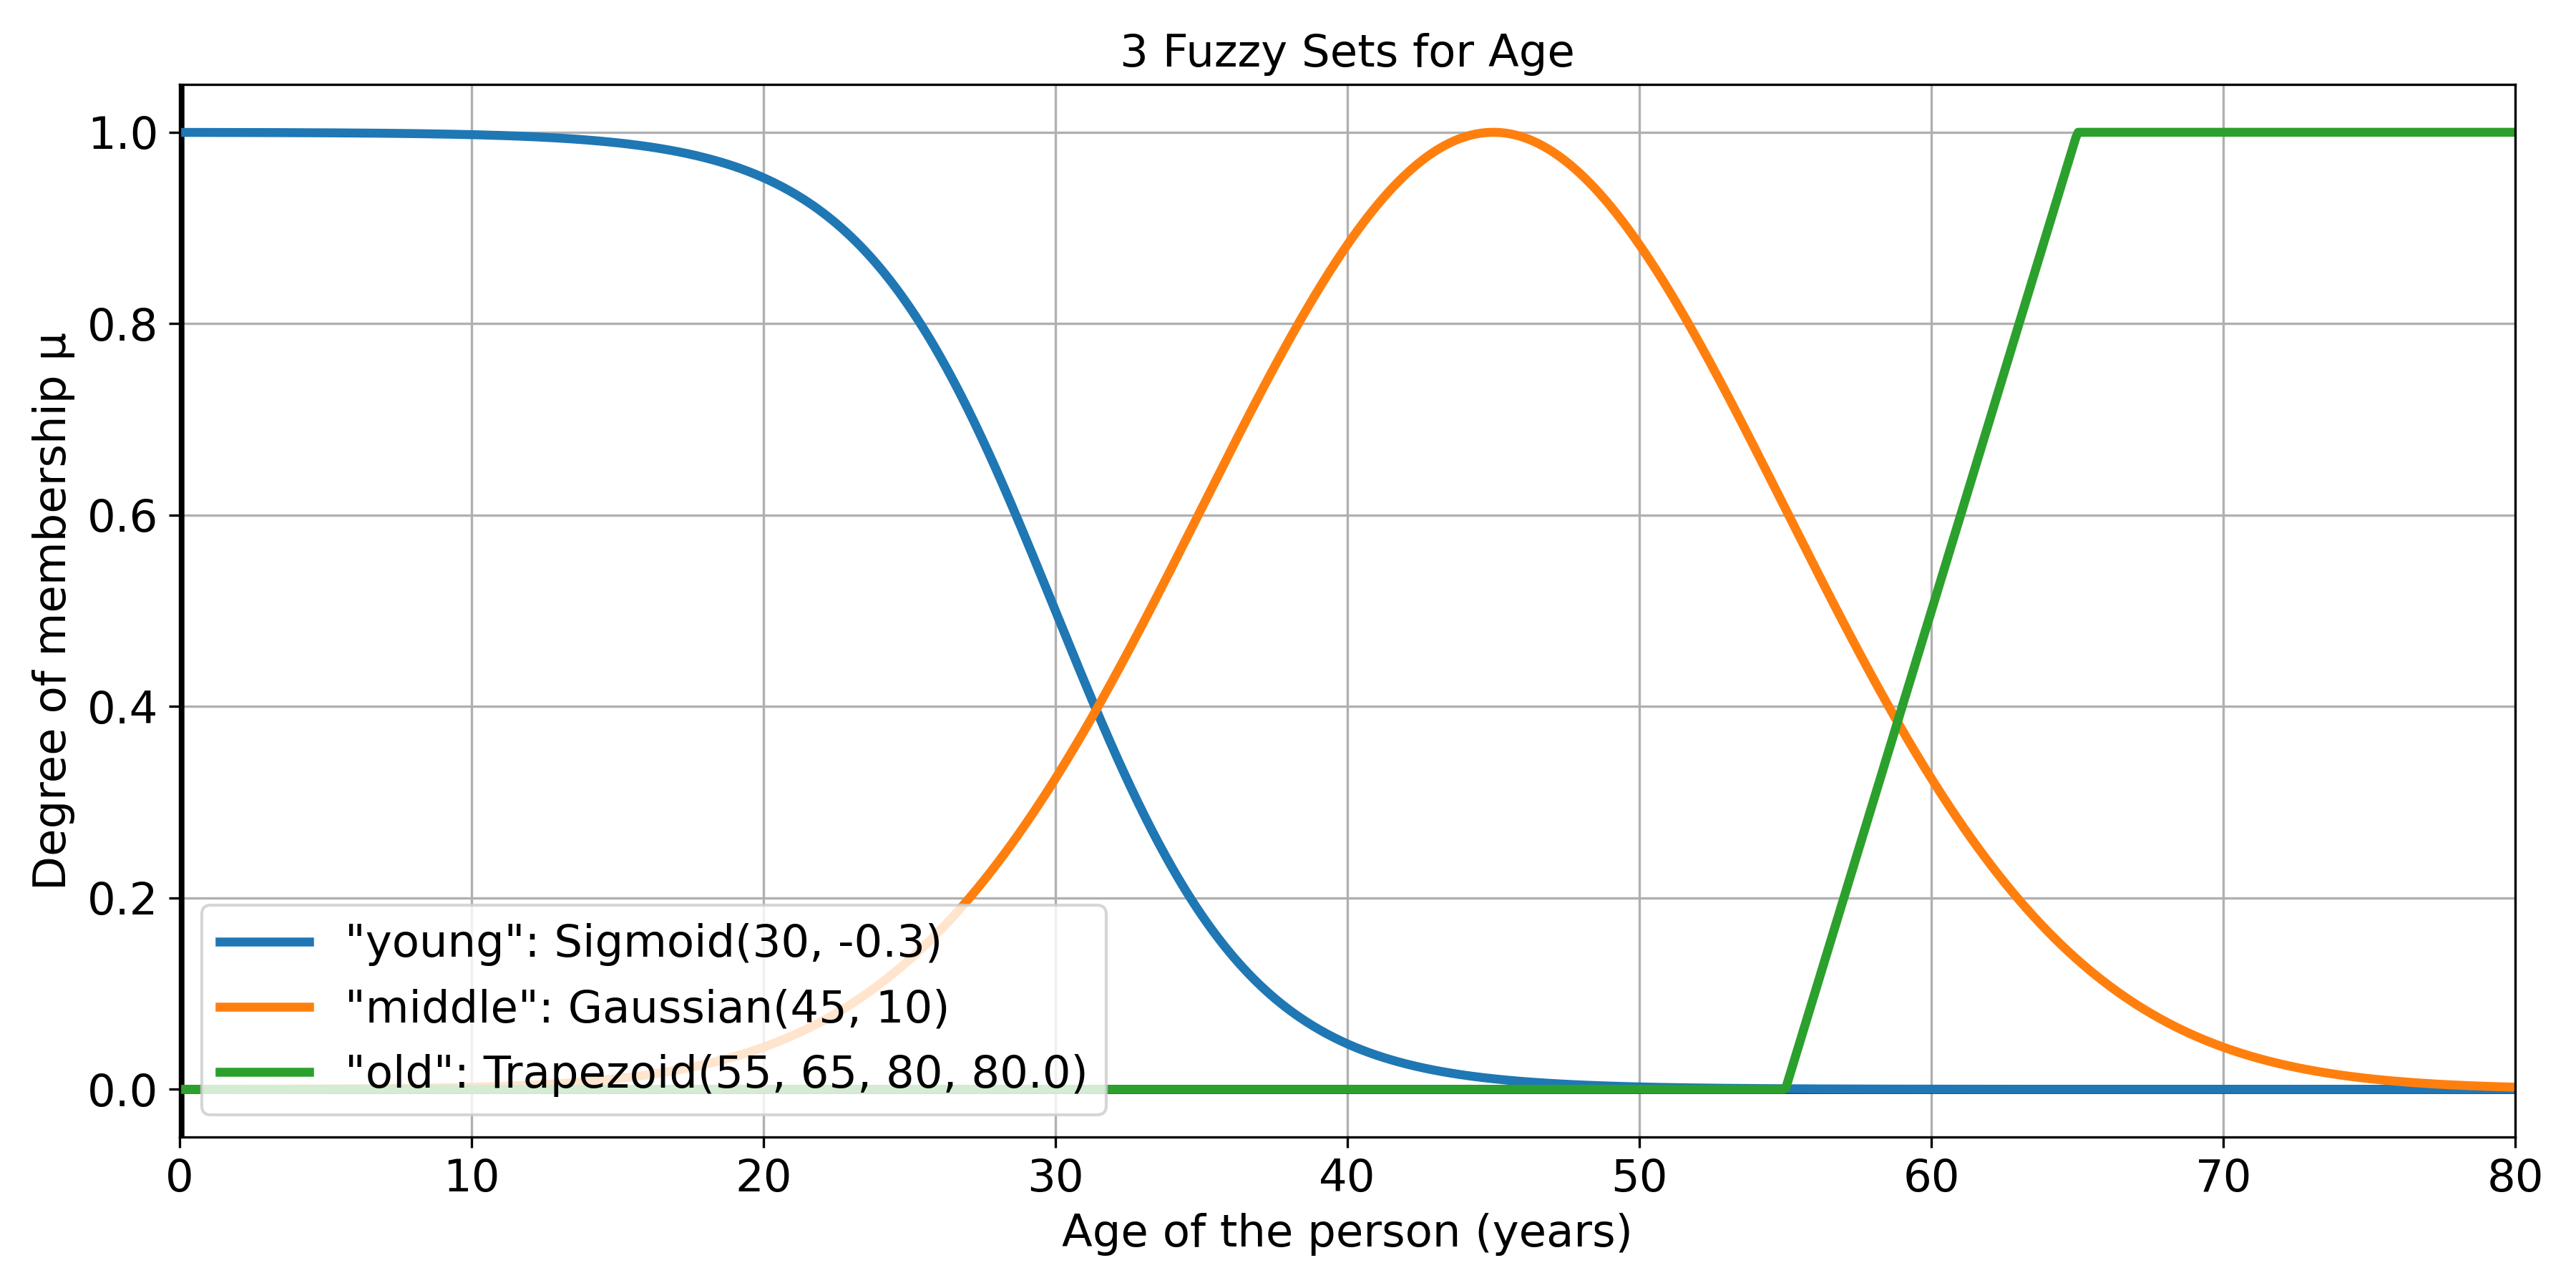
\includegraphics[width=0.8\columnwidth,trim={0 0 0 1cm},clip]{figures/Intro/age-fuzzy-sets.png}
      \caption{Example of fuzzy sets for the age of a person. Fuzzy sets can be used to model the gradual transition between age groups. The distribuitions could be derived from survey data on how people perceive age groups. In this example most people would consider a person middle-aged if they are between 35 and 55, there are however outliers ranging as low as 20 and as high as 70.}
      \label{fig:fuzzy_sets}
\end{figure}

\subsection{Fuzzy Logic Operations}

Fuzzy Sets are a generalization of classical sets, and as such, they also support the classical set operations of union, intersection, and complement. Those operations need to be extended to work with fuzzy sets and need to combine both the semantics of classical sets and the concept of vague membership degrees of fuzzy sets.

The extension of classical operators to the world of fuzzy-sets makes use of so-called De Morgan Triplets. Such a triplet $(\top, \bot, \neg)$ consists of a t-norm $\top : [0, 1] \times [0, 1] \rightarrow [0, 1]$, a t-conorm $\bot : [0, 1] \times [0, 1] \rightarrow [0, 1]$ and a strong complement operator $\neg : [0, 1] \rightarrow [0, 1]$. Those operators generalize the classical logical operators, which are only defined on the binary truth values $\{true, false\}$ to continuous values from the continuous interval $[0, 1]$. $\top$ generalizes the logical AND operator, $\bot$ generalizes the logical OR operator, and $\neg$ generalize the logical NOT operator. Instead of the binary functions used in classical logic, those new operators are continuous functions implementing mappings between degrees of truth.

The binary operators $\top$ and $\bot$ are often written in infix notation as $a \; \top \; b$ and $a \; \bot \; b$, similar to how classical logical operators are written.

For the t-norm $\top$ to be valid, it needs to satisfy the following properties:

\begin{align*}
      a \; \top \; b                & = b \; \top \; a                                              & \quad \text{//Commutativity}    \\
      a \; \bot \; b                & \leq c \; \top \; d  \quad \text{if }  a\leq b \land b \leq d & \quad \text{//Monotonicity}     \\
      a \; \top \; (b \; \top \; c) & = (a \; \top \; b) \; \top \; c                               & \quad \text{//Associativity}    \\
      a \; \top \; 1                & = a                                                           & \quad \text{//Identity Element}
\end{align*}

The complement operator $\neg$ needs to satisfy the following properties:

\begin{align*}
      \neg 0             & = 1                       & \quad \text{//Boundary Conditions} \\
      \neg 1             & = 0                       & \quad \text{//Boundary Conditions} \\
      \neg y \leq \neg x & \quad \text{if } x \leq y & \quad \text{//Monotonicity}
\end{align*}

Additionally, it is called a strong complement operator if it satisfies the following properties:


The standard negation operator $\neg x = 1 - x$ is a strong complement operator as it satisfies all the properties above and is the most common choice for the negation operator in practice.

Some common choices for t-norms and t-conorms used in practice are shown in Table~\ref{tab:tnorms}.





\begin{table}[H]
      \centering
      {\renewcommand{\arraystretch}{1.2}
            \begin{tabular}{|c|c|c|c|}
                  \hline
                  T-Norm Name & T-Norm   $a \top b$                                                                              & Corresponding T-Conorm      $a \bot b$                                                           \\
                  \hline
                  Minimum     & $\min(a, b)$                                                                                     & $\max(a, b)$                                                                                     \\
                  Product     & $a \cdot b$                                                                                      & $a + b - a \cdot b$                                                                              \\
                  Lukasiewicz & $\max(0, a + b - 1)$                                                                             & $\min(1, a + b)$                                                                                 \\
                  Drastic     & $\begin{cases} b & \text{if } a = 1 \\ a & \text{if } b = 1 \\ 0 & \text{otherwise} \end{cases}$ & $\begin{cases} b & \text{if } a = 0 \\ a & \text{if } b = 0 \\ 1 & \text{otherwise} \end{cases}$ \\
                  Einstein    & $\frac{a \cdot b}{2 - (a + b - a \cdot b)}$                                                      & $\frac{a + b}{1 + a \cdot b}$                                                                    \\

                  \hline
            \end{tabular}
      }
      \caption{Common t-Norms and corresponding t-Conorms concerning the standard negation operator $\neg x = 1 - x$}
      \label{tab:tnorms}
\end{table}

In the following sections, we will only consider the standard negation operator, the minimum t-norm, and the maximum t-conorm, as they are the most common choices in practice in fuzzy logic systems.

With these choices of t-norms, t-conorms, and negation operators, it is possible to define the classical set operations of union, intersection, and complement for fuzzy sets:


\begin{itemize}

      \item \textbf{Intersection} \\
            By expanding the definition of the classical set operation $\cap$ using its boolean form $x \in A \cap B \; \iff \; x \in A \; \land \; x \in B$ we can directly translate this to the fuzzy set intersection operation using the t-norm $\top$. The resulting membership function is given by $\mu_{\tilde{A} \cap \tilde{B}}(x) = \mu_{\tilde{A}}(x) \; \top \; \mu_{\tilde{B}}(x)$. Using the minimum t-norm, the intersection of two fuzzy sets $\tilde{A}$ and $\tilde{B}$ is described by the following membership function:

            \begin{equation*}
                  \mu_{\tilde{A} \cap \tilde{B}}(x) = \min(\mu_{\tilde{A}}(x), \mu_{\tilde{B}}(x))
            \end{equation*}


      \item \textbf{Union} \\
            By expanding the definition of the classical set operation $\cup$ using its boolean form $x \in A \cup B \; \iff \; x \in A \; \lor \; x \in B$ we can directly translate this to the fuzzy set union operation using the t-conorm $\bot$. The resulting membership function is given by $\mu_{\tilde{A} \cup \tilde{B}}(x) = \mu_{\tilde{A}}(x) \;\bot \; \mu_{\tilde{B}}(x)$. Using the maximum t-conorm, the union of two fuzzy sets $\tilde{A}$ and $\tilde{B}$ is described by the following membership function:

            \begin{equation*}
                  \mu_{\tilde{A} \cup \tilde{B}}(x) = \max(\mu_{\tilde{A}}(x), \mu_{\tilde{B}}(x))
            \end{equation*}

      \item \textbf{Complement} \\
            By again expanding the classical set operation $A^c$ using its boolean form $x \in A^c \; \iff \; \neg (x \in A)$ we can directly translate this to the fuzzy set complement operation using the negation operator $\neg$. The resulting membership function is given by $\mu_{ \tilde{A}^c}(x) = \neg \mu_{\tilde{A}}(x)$. Using the standard negation operator, the complement of a fuzzy set $\tilde{A}$ is described by the following membership function:

            \begin{equation*}
                  \mu_{ \tilde{A}^c}(x) = 1 - \mu_{\tilde{A}}(x)
            \end{equation*}
\end{itemize}

\todo{add grafical representation of the operations}

\subsection{Linguistic Variables}

Linguistic variables collect multiple fuzzy sets defined over the same crisp set $X$ into a single object. This variable then allows us to reason about the possible states of the variable more naturally.

For example, the linguistic variable "temperature" might have the linguistic terms \emph{cold} \emph{warm}, and \emph{hot}, each of which is defined by a fuzzy set. This representation is very natural as it abstracts away the specific temperature values and allows us to reason about the temperature in a more human-like way.

All the underlying fuzzy sets can be chosen arbitrarily and can also overlap with each other.

\todo{add grafical representation of the linguistic variable}

\subsection{Fuzzy Logic Rules}

Fuzzy Logic Rules are a way to encode expert knowledge into a Fuzzy Logic system. The rules specify the relationship between input and output variables of the system and, therefore, are the backbone of fuzzy logic systems.
The rules are typically encoded in a human-readable way and often have the form "$\text{IF} \; \text{antecedent} \; \text{THEN} \; \text{consequent}$" where both the antecedent and the consequent are fuzzy sets. The antecedent is a condition that must be satisfied for the rule to be applied, while the consequent is the action taken if the rule is applied. Since we are not dealing with binary truth values, the antecedent can only be partially satisfied, and consequently, the rule is only partially applied.

The antecedent can be arbitrarily complicated and involve multiple fuzzy sets and logical operators. The consequent is typically a single fuzzy set modified by the rule but could theoretically be arbitrarily complicated. In this work, we allow rules following the grammar defined below:

%makro for fuzzy set
\newcommand{\fuzzyset}{\langle \text{fuzzy set} \rangle}

\newcommand{\fuzzyrule}{\langle \text{rule} \rangle}


\begin{align*}
      \fuzzyrule  ::= & \ \ \text{IF} \ \fuzzyset \ \text{THEN} \ \fuzzyset & \text { //Rule}        \\[10pt]
      \fuzzyset  ::=  & \ \ (\; \fuzzyset \;)                               & \text { //Parentheses} \\
                      & |  \ \fuzzyset \ \text{AND}  \ \fuzzyset            & \text { //Conjunction} \\
                      & |  \ \fuzzyset \ \text{OR} \  \fuzzyset             & \text { //Disjunction} \\
                      & |  \ \text{NOT} \ \fuzzyset                         & \text { //Negation}    \\
                      & |  \ \tilde{A} \ =\ a                               & \text { //Selection}   \\
\end{align*}

The boolean operators AND, OR, and NOT represent the set operations of intersection, union, and complement, respectively.


Using this grammar, a typical rule might look like this:

\begin{equation}
      \text{IF} \;( \tilde{A} = a \; \text{AND} \; \tilde{B} = b )\; \text{THEN} \; \tilde{C} = c
\end{equation}

This rule states that if the state of the linguistic variable $A$ is $a$ and the state of the linguistic variable $B$ is $b$, then the state of the linguistic variable $C$ should be $c$. However, contrary to classical logic, the rule does not have to activate fully but can have a degree of activation in the interval $[0, 1]$. Should the antecedent be only partially true (for example, if $\mu_{\tilde{A}}(a) = 0.8$ and $\mu_{\tilde{B}}(b) = 0.6$), the rule is only partially applied and the effect of adapting the consequent is reduced accordingly? In the example above, the degree of activation of the rule would be $\min(0.8, 0.6) = 0.6$.

The inference step can be seen as an extension of the boolean implication operator

\[\text{IF} \; \text{antecedent} \; \text{THEN} \; \text{consequent} \iff \text{antecedent} \implies \text{consequent}\]

Moreover, it could be deduced from the choice of the t-norm and t-conorm operators and would lead to $(a \implies b) = \neg a \lor b = \max(1-a,b)$. However, the Mamdani implication is typically used as the AND operation $\min(a,b)$. From a logical point of view, this choice is counterintuitive as it violates the standard definition. However, in the context of fuzzy systems, it is a perfect choice for computing the degree of validity for a rule~\cite {BouchonMeunier1995}. In practice, we are not interested in the resulting fuzzy set of the implication but rather in the extent to which the consequent should be adapted. Therefore, we introduce a slightly different inference algorithm:

\vspace{1em}

Consider the rule $\text{IF} \; \tilde{A} = a \; \text{THEN} \; \tilde{C} = c$

\begin{enumerate}
      \item Obtain the input values $(x_1, x_2, \ldots, x_n) \in X_{A}$ occuring in the crisp set of the antecedent.
      \item Evaluate the degree of membership $\mu$ those input values have in the antecedent. This is the degree to which the antecedent is satisfied, and the rule is activated.
      \item Define a new fuzzy set $R=\tilde{C}\uparrow \mu$ where $\uparrow$ is the cut operator.
            This operator is defined as $\mu_{R}(x) = \min(\mu_{\tilde{C}}(x), \mu)$, which means that it cuts off all membership values of the fuzzy set $\tilde{C}$ that are above the degree of activation $\mu$. This resulting set $R$ contains the information to which extent the consequent should be adapted. We see that in the extreme cases where $\mu = 0$, the set $R$ is also empty and does not affect further computations. If $\mu = 1$, the rule is activated fully, and the set $R$ is equal to $\tilde{C}$. In all other cases, the set $R$ is trimmed to the extent of activation.
\end{enumerate}

\subsection{Defuzzification}

The final step in a Fuzzy Logic system is the defuzzification step. In this step, the fuzzy output of the system is converted back into a crisp value that can be used to control natural-world systems. The first step in defuzzification is to collect all the rules operating on the same output variable and combine their trimmed consequents into a single fuzzy set. This is done by just taking the fuzzy union of all those consequences, which results in a new fuzzy set that represents the combined effect of all the rules on the output variable. This fuzzy set can be converted back into a single crisp value representing some aspect of the fuzzy set using a defuzzification method.

There are many different ways to defuzzify a fuzzy set. Some of the most common methods are:

\begin{itemize}
      \item \textbf{Centroid} \\
            The Centroid method calculates the center of mass of the fuzzy set and returns this value as the crisp output. This method is intuitive as it tries to find a weighted interpolation of all the activated fuzzy sets. It is defined as:

            \begin{equation}
                  \text{Centroid} = \frac{\int_X x \cdot \mu_{\tilde{C}}(x) \, dx}{\int_X \mu_{\tilde{C}}(x) \, dx}
            \end{equation}

      \item \textbf{Mean of Maximum} \\
            The Mean of Maximum method calculates all the input values that result in the maximum membership value of the fuzzy set and returns the average of these values as the crisp output. When there is just one maximum value, this method can be thought of as just returning the x-position of the most likely value.

            It is defined as follows:

            \begin{equation}
                  \text{Mean of Maximum} = \frac{\int_{X'} x \, dx}{\int_{X'}  \, dx}
            \end{equation}
            where $X' = \{x \in X \, | \, \mu_{\tilde{C}}(x) = \max(\mu_{\tilde{C}}(x))\}$ is the set of all input values that result in the maximum membership value of the fuzzy set.



      \item \textbf{Weighted Average} \\
            The Weighted Average method calculates the average of all the input values weighted by their membership values. Contrary to the Centroid method, which integrates over the whole domain, the Weighted Average method only considers a singular point from each membership function where the membership value is maximal. This can be seen as a simplification of the Centroid method and is defined as:

            \begin{equation}
                  \text{Weighted Average} = \frac{\sum_{x \in X'} x \cdot \mu_{\tilde{C}}(x)}{\sum_{x \in X'} \mu_{\tilde{C}}(x)}
            \end{equation}
            where $X'$ is the set of all input values resulting in their fuzzy set's maximum membership value.
\end{itemize}

Also, many other methods exist to defuzzify a fuzzy set, but the ones mentioned above are the most common choices in practice. This thesis focuses on the Centroid and the Mean of Maximum methods.


\subsection{Structure of creating a Fuzzy Logic System}

All the building blocks of a Fuzzy Logic System have been introduced in the previous sections and can now be combined to create a complete Fuzzy Logic System. The general structure of a Fuzzy Logic System is as follows:

\begin{enumerate}
      \item \textbf{Fuzzification} \\
            The first step in a Fuzzy Logic System is to convert the crisp input values into fuzzy sets. This is done by evaluating the membership functions of the fuzzy sets at the crisp input values. This results in a bunch of membership values, which can be used to calculate the boolean operations of the antecedents of the rules.

      \item \textbf{Inference} \\
            The next step is to apply the fuzzy logic rules to the fuzzy input values. This is done by using the degree of membership of the input values in the rules' antecedents to calculate each rule's activation degree. The consequent of each rule is then cut by the degree of activation of the rule to determine the effect of the rule on the output variable. This results in many fuzzy sets representing all the active effects on the output variable.

      \item \textbf{Aggregation} \\
            The fuzzy sets resulting from the inference step are combined into a single fuzzy set containing the combined effect of all the rules on the output variable. This is done by taking the fuzzy union of all the fuzzy sets.

      \item \textbf{Defuzzification} \\
            The final step is to convert the fuzzy output value into a crisp value that can be used to control natural-world systems. This is done by applying a defuzzification method to the fuzzy set representing the combined effect of all the rules on the output variable.
\end{enumerate}


If the system is finished, it can be seen as a black box that takes crisp input values and returns crisp output values similar to a function $f: X \rightarrow \mathbb{R}$.


Using such a system, however, requires much expert knowledge as the rules and the membership functions of the fuzzy sets need to be defined by hand. This can be time-consuming and sometimes even impossible if the system is too complex. Luckily, other methods exist that attempt to automate defining the parameters of the fuzzy logic system. Some standard methods are:

\begin{itemize}
      \item \textbf{Genetic Algorithms} \\
            Genetic Algorithms are a class of optimization algorithms that are inspired by the process of natural selection. They maintain a population of candidate solutions to a problem and iteratively improve them by applying genetic operators such as mutation and crossover. Genetic Algorithms can optimize the parameters of a fuzzy logic system by treating the parameters as an individual's genes and the system's performance as the individual's fitness. By iteratively evolving the population of individuals, it is possible to find a set of parameters that optimizes the performance of the fuzzy logic system.

      \item \textbf{Data Driven Methods} \\
            Data Driven Methods are a class of optimization algorithms that work by using data to optimize the parameters of a fuzzy logic system. Those methods are often based on machine learning algorithms such as decision trees. They work by trying to find some interpretable representation of the data that can be used to define concrete rules for the fuzzy logic system.

      \item \textbf{Fuzzy Clustering} \\
            Fuzzy Clustering is a class of clustering algorithms that work by assigning each data point to a cluster with a certain degree of membership. It can be used to optimize the parameters of a fuzzy logic system by treating the data points as the input values of the system and the clusters as the fuzzy sets of the system. By iteratively updating the clusters to better fit the data points, it is possible to find a set of parameters that optimizes the performance of the fuzzy logic system.
            \todo{find sources for all of them}
\end{itemize}